%% Introduction
\section{Introduction}
\lettrine[lines=2]{A}{ctive} Noise Control (ANC) is a used technique in a wide variety of applications. Research is being done in creating silents zones\cite{SilentZones}, Improving room acoustics using multiple loudspeakers\cite{CAPS} and is already available in various headphones, for noise cancellation, both for professional and consumer use. 

Noise canceling headphones are used in various environments which have different noise characteristics. These characteristics vary from periodic low frequency noise (60-400Hz), e.g. from machinery and helicopter rotor\cite{LowFrequency}, med-range frequency noise (100-4000Hz), e.g. speech\cite{MidFrequency}, to high frequency noise (8-12 Hz), e.g. turbine noise\cite{LowFrequency}. The high frequency noise is naturally attenuated by using a closed headphone cup\cite{naturalAttenuation} and static low frequency noise are attenuated by the present consumer headphones\cite{ConsumerANC}.
%\footnote{Numbers and sources will be added to the statements}.   
%%ANC are used by companies such as Bang \& Olufsen and Lyngdorf Audio in their proprietary technology as Active Room Compensation\texttrademark and RoomPerfect\texttrademark respectively, to control noise in a room using loudspeakers. Headphone industries have adapted it into cancellation of noise and is used 

\begin{figure}[H]
	\centering
	\textbf{\textit{Here is going to be a graph of different}}
	\textbf{\textit{ headphones tested with non stationary signals (Speech)}}
	\caption{Figure in the making}
\end{figure}


Assuming speech as the primary noise source, the solution used in this paper as a reference is a digital feedforward system using the Filtered-X Least Mean Squares (FXLMS). The solution is chosen due to it being the optimal system for non stationary signals. The general solutions in ANC are described thoroughly by Hansen et al. \cite{Hansen2}, \cite{Hansen}.

The problem of a feedforward system is the dependency of noise having a propagation delay from the noise source the source. 

{
	\centering
	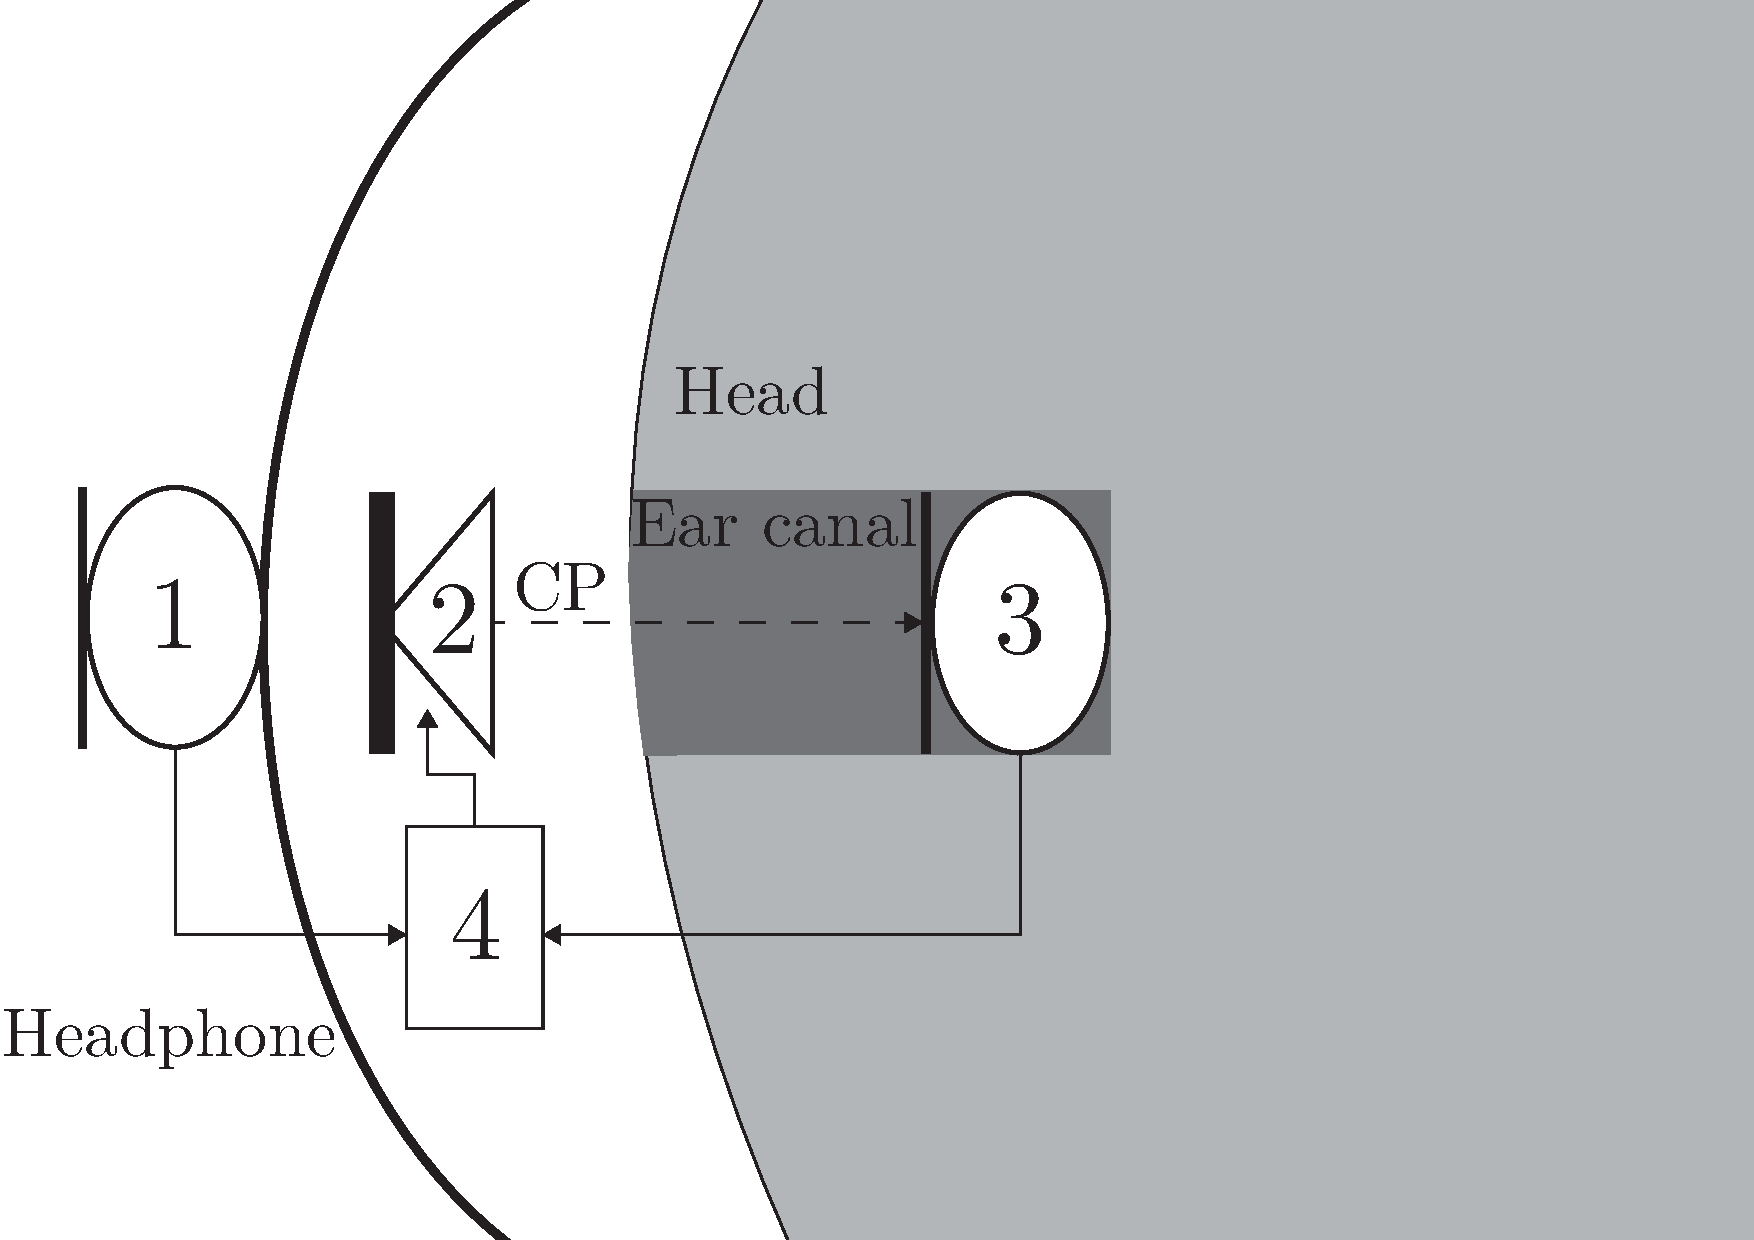
\includegraphics[width=0.5\columnwidth]{figures/ArticleIllustrations/BasicOverviewZoomed}
	\captionof{figure}{Simplified ANC Headphone on ear. Showing the outer reference microphone (1), a headphone loudspeaker (2), an error microphone (3) and a DSP (4).}
	\label{fig:SystemOverview}
}

A parameter in ANC is the bandwidth which is determined by the system delay, introduced by sampling and processing the signal in the feedforward system. Consumer ANC headphones has a bandwidth that does not cover the entire frequency area of speech. This paper examines how to extend the bandwidth.

To increase bandwidth a prediction algorithm is proposed as a potential solution. In order to do prediction, certain signal characteristics must be known. Prediction of speech is described by Wai C. Chu \cite{Speech}. In this paper we will combine the reference solution with the prediction of speech to increase the bandwidth of a real time system.  

The paper is split into two parts. The first part describes the method used in the reference solution and how to predict speech using Linear Prediction (LP). The second part describes simulations and the implementation. Performance of the reference and the combined solution are determined and the increase in performance of the LP ANC system is verified.  
        
%why performance decreases with increased frequency and



%  The scope of this paper is not to derive a new ANC algorithm, but rather to expand the existing FXLMS algorithm by prediction. The goal of this modification is to achieve increased performanec, especially at higher frequencies.\\
% The application of the system is cancellation of speech in a call centre. The choice of a specific use case allows the frequency range and signal type of interest to be defined before designing the system. Call centres is an especially interesting environment for an ANC system, because the unwanted noise and the wanted signal have the same  characteristics as they are both speech. \\
% The paper is split into three parts. The first part examines the demands for an ANC system to be used in a call centre. The second part discus the algorithm used and shows preliminary results from simulations. The third part describes the real time implementation of the algorithm and verifies the performance of the ANC system.  




% \lettrine[lines=2]{A}{ctive} Noise Control (ANC) is a field of study, where a lot of algorithms are already known. The scope of this paper is not to derive a new ANC algorithm, but rather to expand the existing FXLMS algorithm by prediction. The goal of this modification is to achieve increased performanec, especially at higher frequencies.\\
% The application of the system is cancellation of speech in a call centre. The choice of a specific use case allows the frequency range and signal type of interest to be defined before designing the system. Call centres is an especially interesting environment for an ANC system, because the unwanted noise and the wanted signal have the same  characteristics as they are both speech. \\
% The paper is split into three parts. The first part examines the demands for an ANC system to be used in a call centre. The second part discus the algorithm used and shows preliminary results from simulations. The third part describes the real time implementation of the algorithm and verifies the performance of the ANC system.  




%\lettrine[lines=2]{A}{ctive} Noise Control (ANC) is a field of study, where a lot of algorithms are already known. \todo[inline]{$MENTION A FEW$} The scope of this paper is not to derive a new ANC algorithm, but rather to use an existing algorithm in a practical application. The application is cancellation of speech in a call centre The choice of a specific use case allows the frequency range and signal type of interest to be defined before designing the system. Call centres is an especially interesting environment for an ANC system, because the unwanted noise and the wanted signal have the same  characteristics as they are both speech. \\
%The paper is split into three parts. The first part examines the demands for an ANC system to be used in a call centre. The second part discus the algorithm used and shows preliminary results from simulations. The third part describes the real time implementation of the algorithm and verifies the performance of the ANC system.  